% For PRD: \documentclass[aps,prd,twocolumn,superscriptaddress,nofootinbib]{revtex4-2}
\documentclass[10pt,twocolumn]{article}
\usepackage[a4paper,margin=1.9cm,columnsep=0.7cm]{geometry}
\usepackage{amsmath,amssymb}
\usepackage{booktabs,multirow}
\usepackage{graphicx}
\usepackage[numbers,sort&compress]{natbib}
\usepackage[hidelinks]{hyperref}
\usepackage{xcolor}
\newenvironment{acknowledgments}{\section*{Acknowledgments}}{}
\newcommand{\Bc}{B_c}
\newcommand{\Bcs}{B_c^*}
\newcommand{\cc}{c\bar c}
\newcommand{\bb}{b\bar b}
\newcommand{\cb}{c\bar b}
\newcommand{\MeV}{\,\mathrm{MeV}}
\newcommand{\GeV}{\,\mathrm{GeV}}
\newcommand{\GeVi}{\,\mathrm{GeV}^{-1}}
\graphicspath{{figures/}}

\begin{document}

\twocolumn[
\begin{@twocolumnfalse}
\begin{center}
{\LARGE\bfseries What does the quarkonium spectrum know about the heavy-quark potential?}

\vspace{2pt}
{\large A model-independent extraction of $V(r)$ from charmonium and bottomonium, and its consequences for $\Bc$}

\vspace{10pt}
{\large Peter Agyemang Oppong}

\vspace{2pt}
{\small\itshape School of Physics and Astronomy, University of Glasgow, Glasgow G12 8QQ, United Kingdom}

\vspace{2pt}
{\small \today}
\end{center}
\begin{quote}\small
We determine the static heavy-quark potential $V(r)$ directly from the measured charmonium and bottomonium spectra, without assuming a functional form.
$V(r)$ is represented by a cubic spline with up to twelve knots on $0.15\le r\le8\GeVi$ plus a Coulomb term, and is fitted together with the quark masses and a running coupling to 27 $J$-resolved $\cc$ and $\bb$ levels from the 2026 Review of Particle Physics, with a smoothness prior whose strength is scanned.
The result is a potential with a one-standard-deviation band: $V(r)$ is determined to $30$--$50\MeV$ for $0.7\lesssim r\lesssim7\GeVi$, to $100$--$300\MeV$ for $0.2\lesssim r\lesssim0.5\GeVi$, and not at all below $0.2\GeVi$, where the spectrum has no sensitivity and the short-distance form is fixed only through the hyperfine splittings.
The band is stable against the number of knots and the prior strength and the fit quality ($\chi^2=40$ for 27 levels) is better than that of any parametric form.
Compared at equal shape, the logarithmic and power-law potentials lie within the band everywhere, whereas the Cornell potential is excluded at three standard deviations at $r\simeq3\GeVi$.
Propagated to $\cb$, the extraction gives $\Bc$ masses with uncertainties of $4$--$5\MeV$ that are independent of the choice of potential: $\Bc(1S)=6264\pm5$, $\Bcs(1S)=6336\pm6$, $\Bc(2S)=6874\pm5\MeV$, in agreement with ATLAS for $\Bcs$ and with the measured $2S$, but $10\MeV$ low for the ground state, so that the $2S$--$1S$ spacing of $\Bc$ is predicted $12\pm7\MeV$ larger than measured. This is the only place where the $\cb$ system departs from the potential determined by $\cc$ and $\bb$, and it cannot be removed by any change of the potential's shape.
\end{quote}
\vspace{6pt}
\end{@twocolumnfalse}
]

% ===========================================================================
\section{Introduction}
\label{sec:intro}

Non-relativistic potential models describe the spectra of charmonium and bottomonium to a few tens of MeV, and have done so for fifty years with a handful of parametric forms~\cite{Eichten1978,Quigg1977,Martin1980,Buchmuller1981,Godfrey1985}.
The question we ask here is the inverse one: given the spectra, what is actually known about $V(r)$?
Which distances are constrained, by which states, and how well?
The question has a practical side.
Predictions for states that have not been measured---the $P$ and $D$ waves of $\Bc$, the higher bottomonia---are quoted with a ``model dependence'' estimated by comparing a few parametric potentials.
That estimate is as arbitrary as the choice of potentials.
A potential extracted from the data with a proper error band turns the model dependence into a derived quantity.

There is a well-known answer to a related question: the static potential computed in lattice QCD~\cite{Bali2001} and the phenomenological fits agree in the range $0.2\lesssim r\lesssim1\,$fm, i.e.\ $1\lesssim r\lesssim5\GeVi$, where the potentials of Refs.~\cite{Eichten1978,Quigg1977,Martin1980} nearly coincide despite their different functional forms~\cite{Kiselev2001}.
What has not been done, to our knowledge, is to let the spectrum itself determine $V(r)$ with current data, including the spin-dependent levels and the $D$ waves, and to quantify the result with a covariance.
That is the content of this paper.

Our method is a flexible (spline) representation of $V(r)$ fitted by least squares with a smoothness prior, which is the standard approach to ill-posed inverse problems and gives a covariance for the function.
We apply it to the data set and spin-dependent treatment of a companion paper on $\Bc$~\cite{Oppong2026}, so that the two analyses can be compared directly.
Section~\ref{sec:method} describes the parametrisation and the fit, Sec.~\ref{sec:results} the extracted potential and its sensitivity, Sec.~\ref{sec:bc} the consequences for $\Bc$, and Sec.~\ref{sec:conclusions} concludes.

% ===========================================================================
\section{Method}
\label{sec:method}

\subsection{Flexible potential}

We write
\begin{equation}
  V(r) = -\frac{\kappa}{r} + S(r),
  \label{eq:V}
\end{equation}
where $S$ is a natural cubic spline in $x=\ln r$ through $K$ knots log-spaced on $[0.15, 8]\GeVi$, the range occupied by the wave functions of the fitted states (from the inner 1\% of the $\bb$ $1S$ to the outer 99\% of the $\cc$ $3S$).
Below the first knot $S$ is held constant, so that the Coulomb term alone sets the short-distance behaviour; beyond the last knot $S$ is continued linearly in $r$ with its slope at $8\GeVi$, a string-like extrapolation that affects only states reaching beyond the data.
An additive constant in $V$ is exactly degenerate with $m_c+m_b$; we remove it by fixing the knot at $r=1\GeVi$ so that $V(1\GeVi)=-1.166\GeV$, the value of the Martin potential of Ref.~\cite{Eichten1994}.
The free parameters are the $K-1$ remaining knot values, $\kappa$, $m_c$, $m_b$ and the QCD scale $\Lambda$ of a one-loop running coupling $\alpha_s(\mu)$, $\mu=\sqrt{m_1m_2}$, that enters the spin-dependent terms.
With $K=8$ there are eleven.

Bound states are obtained by integrating the radial Schrödinger equation with the Numerov method and locating eigenvalues by node-counting bisection; fine and hyperfine structure is added in first-order perturbation theory following Eichten and Quigg~\cite{Eichten1994}, with the $J=L$ states of unequal-mass mesons mixed.
These are the methods of Ref.~\cite{Oppong2026}, where they are described in full; the $\Bc$ predictions below are therefore directly comparable to the parametric ones of that paper.

\subsection{Data and fit}

The data are the 27 $J$-resolved charmonium and bottomonium levels below open-flavour threshold listed in Ref.~\cite{Oppong2026} (Table~1 there), taken from the 2026 Review of Particle Physics~\cite{PDG2026}: $\eta_c$, $J/\psi$, the four $1P$ states, $\eta_c(2S)$, $\psi(2S)$, $\psi(3770)$, $\psi_2(3823)$ and $\psi_3(3842)$ for charmonium; $\eta_b$, $\Upsilon(1S)$, the four $1P$ states, $\eta_b(2S)$, $\Upsilon(2S)$, $\Upsilon_2(1D)$, the four $2P$ states, $\Upsilon(3S)$, $\chi_{b1}(3P)$ and $\chi_{b2}(3P)$ for bottomonium.
A theory floor of $10\MeV$ is added in quadrature to the experimental errors.

The residual vector is the 27 data residuals followed by the smoothness prior
\begin{equation}
  \sqrt\lambda\;\frac{s_{k+1}-2s_k+s_{k-1}}{(\Delta x)^2},\qquad k=2,\dots,K-1,
  \label{eq:prior}
\end{equation}
on the knot values $s_k$, and the sum of squares is minimised with a trust-region least-squares algorithm.
The covariance of the parameters is the inverse Gauss--Newton matrix of the full residual vector, so the prior is included in the error band, as it should be: the band quantifies what the data plus the smoothness assumption determine.
The band on $V(r)$ follows from the covariance of the knot values by linear propagation (the spline is linear in them), and vanishes at $r=1\GeVi$ by construction; everywhere else it measures the uncertainty of the shape relative to that point.

The prior strength $\lambda$ and the number of knots $K$ are not fitted.
We scan $K\in\{6,8,10,12\}$ and $\lambda\in\{0.1,1,10,100\}$ and require that the extracted band be stable; we also repeat the reference fit with the $\cc$ $D$ waves or the $\bb$ $3P$ levels removed, with a $5\MeV$ floor, and with $\kappa$ fixed.

% ===========================================================================
\section{The extracted potential}
\label{sec:results}

\begin{figure}[t]
\centering
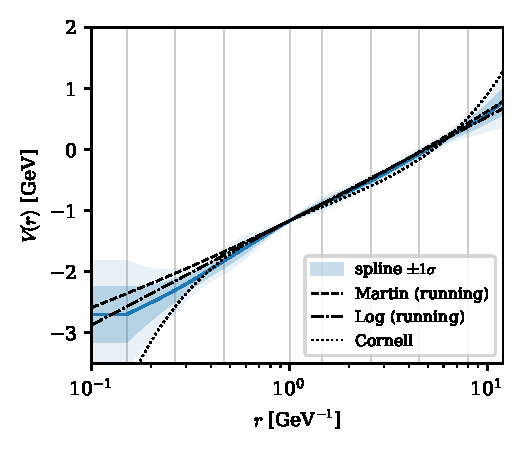
\includegraphics[width=\columnwidth]{figA1_potential_band}
\caption{The potential extracted from the $\cc+\bb$ spectrum ($K=8$, $\lambda=1$): central value with $1\sigma$ (dark) and $2\sigma$ (light) bands. The refitted Martin, logarithmic and Cornell potentials of Ref.~\cite{Oppong2026}, shifted by a constant to $V(1\GeVi)=-1.166\GeV$, are shown for comparison; vertical lines mark the knots.}
\label{fig:band}
\end{figure}

\begin{figure}[t]
\centering
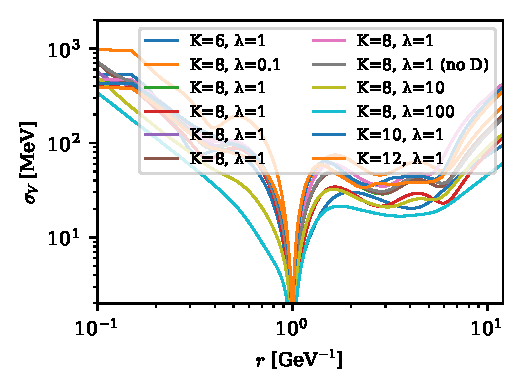
\includegraphics[width=\columnwidth]{figA2_band_width}
\caption{Width of the $1\sigma$ band for all fits in the stability scan. The dip at $r=1\GeVi$ is the anchoring convention.}
\label{fig:width}
\end{figure}

\begin{table}[t]
\caption{The extracted potential (GeV) at selected $r$ for the reference fit, with the three parametric potentials of Ref.~\cite{Oppong2026} shifted to the same value at $r=1\GeVi$.}
\label{tab:V}
\centering\small
\begin{tabular}{lcccc}
\toprule
$r$ [GeV$^{-1}$] & $V\pm\sigma_V$ & Martin & Log & Cornell \\
\midrule
0.2 & $-2.504\pm0.271$ & $-2.192$ & $-2.358$ & $-3.136$ \\
0.3 & $-2.202\pm0.129$ & $-1.949$ & $-2.057$ & $-2.358$ \\
0.5 & $-1.761\pm0.096$ & $-1.629$ & $-1.679$ & $-1.714$ \\
0.75 & $-1.401\pm0.041$ & $-1.362$ & $-1.379$ & $-1.364$ \\
1 & $-1.166\pm0.001$ & $-1.166$ & $-1.166$ & $-1.166$ \\
1.5 & $-0.880\pm0.047$ & $-0.880$ & $-0.866$ & $-0.922$ \\
2 & $-0.688\pm0.040$ & $-0.670$ & $-0.653$ & $-0.754$ \\
3 & $-0.399\pm0.029$ & $-0.363$ & $-0.353$ & $-0.493$ \\
4 & $-0.173\pm0.039$ & $-0.138$ & $-0.140$ & $-0.271$ \\
6 & $+0.153\pm0.036$ & $+0.191$ & $+0.161$ & $+0.136$ \\
8 & $+0.383\pm0.080$ & $+0.433$ & $+0.374$ & $+0.524$ \\
\bottomrule

\end{tabular}
\end{table}

\begin{table*}[t]
\caption{Stability of the extraction. For each fit: data $\chi^2$ (27 levels), prior $\chi^2$, band width $\sigma_V$ (MeV) at four distances, and central $V$ (GeV) at three. Variants: no $D$ ($\cc$ $D$ waves removed), no $3P$ ($\bb$ $3P$ removed), floor 5 (theory floor $5\MeV$), $\kappa$ fixed at $0.3$ or $0.5$.}
\label{tab:stab}
\centering\small
\begin{tabular}{cclcccccccccc}
\toprule
$K$ & $\lambda$ & variant & $\chi^2_{\rm data}$ & $\chi^2_{\rm prior}$ & $\sigma_V(0.3)$ & $\sigma_V(1)$ & $\sigma_V(3)$ & $\sigma_V(6)$ & $V(0.3)$ & $V(3)$ & $V(6)$ \\
\midrule
6 & 1 & -- & 40.6 & 2.2 & 83 & 0 & 24 & 33 & $-2.204$ & $-0.412$ & $+0.149$ \\
8 & 0.1 & -- & 35.6 & 2.5 & 280 & 0 & 46 & 51 & $-2.023$ & $-0.477$ & $+0.092$ \\
8 & 1 & -- & 41.5 & 2.0 & 127 & 0 & 29 & 36 & $-2.197$ & $-0.404$ & $+0.157$ \\
8 & 1 & floor 5 & 150.4 & 10.3 & 100 & 0 & 22 & 23 & $-2.113$ & $-0.442$ & $+0.123$ \\
8 & 1 & $\kappa=0.3$ & 46.6 & 2.1 & 143 & 0 & 29 & 36 & $-2.068$ & $-0.402$ & $+0.158$ \\
8 & 1 & $\kappa=0.5$ & 51.0 & 3.9 & 148 & 0 & 29 & 36 & $-1.968$ & $-0.401$ & $+0.160$ \\
8 & 1 & no $3P$ & 31.7 & 2.4 & 149 & 0 & 35 & 76 & $-2.311$ & $-0.407$ & $+0.211$ \\
8 & 1 & no $D$ & 20.8 & 1.6 & 127 & 0 & 31 & 38 & $-2.235$ & $-0.408$ & $+0.137$ \\
8 & 10 & -- & 46.6 & 2.3 & 78 & 0 & 21 & 28 & $-2.116$ & $-0.370$ & $+0.193$ \\
8 & 100 & -- & 51.3 & 7.4 & 58 & 0 & 17 & 21 & $-2.017$ & $-0.338$ & $+0.220$ \\
10 & 1 & -- & 40.1 & 1.7 & 158 & 1 & 40 & 53 & $-2.133$ & $-0.362$ & $+0.211$ \\
12 & 1 & -- & 40.4 & 1.3 & 124 & 1 & 37 & 47 & $-2.131$ & $-0.363$ & $+0.201$ \\
\bottomrule

\end{tabular}
\end{table*}

Figure~\ref{fig:band} and Table~\ref{tab:V} show the result for the reference fit ($K=8$, $\lambda=1$), which has $\chi^2=41.5$ for the 27 levels with a prior contribution of $2.0$.
This is a better description of the spectrum than any parametric form we have tried: the best of the three families in Ref.~\cite{Oppong2026}, the logarithmic potential with running coupling, has $\chi^2=59$ for the same data, and the Martin potential $70$.
The improvement is not an artefact of the extra freedom: it is the same ($\chi^2=40$--$42$) for $K=6$, $8$, $10$ and $12$ (Table~\ref{tab:stab}), so the data determine a definite shape that six knots already capture and twelve do not over-fit.

\paragraph{Where the potential is known.}
Figure~\ref{fig:width} shows the band width.
$V(r)$ is determined to better than $50\MeV$ over $0.7\le r\le6.9\GeVi$ and to $30$--$40\MeV$ over most of that range; the width grows to $100\MeV$ at $0.3\GeVi$ and $300\MeV$ at $0.2\GeVi$, and the potential is unconstrained below $0.15\GeVi$.
The sensitivity matrix $\partial E_i/\partial s_k$ (Fig.~\ref{fig:sens}) makes the origin of this explicit.
Every level responds mainly to the two or three knots nearest its mean radius: the $\bb$ $1S$ to $0.5\GeVi$, the $\bb$ $1P$ and $\cc$ $1S$ to $1.5\GeVi$, the $\cc$ $1P$ and $\bb$ $2S$, $1D$, $2P$ to $2.6\GeVi$, the $\cc$ $2S$, $D$ waves and $\bb$ $3S$, $3P$ to $4.5\GeVi$.
No level has more than 3\% sensitivity to the knots at $0.15$ and $0.26\GeVi$.
The quarkonium spectrum is blind to the Coulomb region.

\paragraph{The short-distance region and the hyperfine splittings.}
That blindness has a consequence for $\kappa$.
In the reference fit $\kappa$ runs to zero, and fixing it to $0.3$ or $0.5$ (the one-gluon-exchange value $\tfrac43\alpha_s$ for $\alpha_s\simeq0.25$--$0.4$) worsens $\chi^2$ to $47$ and $51$ while leaving $V(r)$ for $r>0.5\GeVi$ unchanged within the band (Table~\ref{tab:stab}).
The spectrum is not pushing $\kappa$ down---it cannot see it; the hyperfine splittings are.
In first-order perturbation theory the $S$-wave hyperfine splitting is proportional to $|R(0)|^2$, which a Coulomb singularity enhances, and the fit lowers $\kappa$ to reduce the over-predicted $\cc$ splitting.
This is the same tension between the $\cc$ and $\bb$ hyperfine splittings found in Ref.~\cite{Oppong2026} with parametric potentials, now isolated to the one region of $V(r)$ that the spin-averaged spectrum does not constrain.
The short-distance form of the potential is therefore an input, not an output, of this analysis; we carry $\kappa\in[0,0.5]$ as a systematic.

\paragraph{Comparison with parametric forms.}
Because an additive constant is absorbed by the quark masses, parametric potentials must be compared at equal shape: in Fig.~\ref{fig:band} and Table~\ref{tab:V} each has been shifted to $V(1\GeVi)=-1.166\GeV$.
So compared, the Martin and logarithmic potentials lie within $1$--$1.5\sigma$ of the extracted band at every $r$ between $0.3$ and $8\GeVi$; their small difference in curvature is below the resolution of the data.
The Cornell potential is different: its linear rise is too steep at intermediate distances, $V(3\GeVi)=-0.498\GeV$ against the extracted $-0.404\pm0.029$, a $3.2\sigma$ deviation that persists ($-0.408$) when the $D$ waves are removed, and its Coulomb term is too strong at $0.2\GeVi$ ($2.3\sigma$).
This is the quantitative version of the long-standing observation that a linear-plus-Coulomb form fits the heavy quarkonia less well than an effective power $r^{0.1}$ or a logarithm~\cite{Martin1980,Eichten1994}: the data require the slope of the confining part to fall with distance, from $dV/dr=0.45\GeV^2$ at $1.5\GeVi$ to $0.25\GeV^2$ at $3\GeVi$ and $0.13\GeV^2$ at $6\GeVi$, whereas a linear term has a constant slope and must compromise between the two ends.

\begin{figure*}[t]
\centering
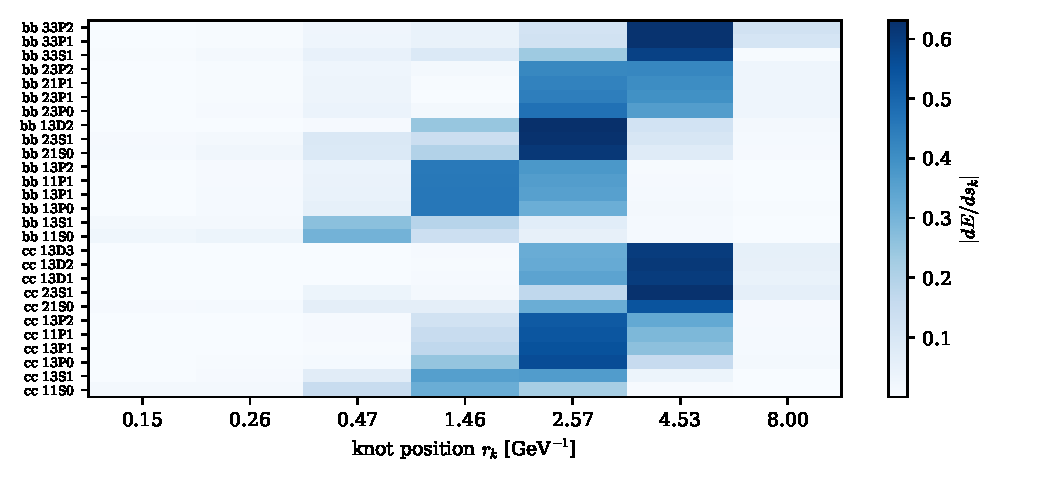
\includegraphics[width=0.9\textwidth]{figA3_sensitivity}
\caption{Sensitivity of each fitted level to the free knot values, $|\partial E_i/\partial s_k|$, for the reference fit. Rows are the 27 levels (charmonium below, bottomonium above), columns the knots.}
\label{fig:sens}
\end{figure*}

\paragraph{Stability.}
Table~\ref{tab:stab} summarises the scan.
Increasing $\lambda$ from $0.1$ to $10$ changes $V(3\GeVi)$ by $0.1\GeV$ and $\chi^2$ from $36$ to $47$; at $\lambda=100$ the prior term ($\chi^2_{\rm prior}=7$) is no longer negligible and the fit is over-regularised, so we exclude it.
Within $0.1\le\lambda\le10$ the band widths at $r\ge1\GeVi$ vary by less than a factor of two and the central values by less than one band width.
Removing the $D$ waves or the $3P$ levels moves $V(r)$ by at most $0.02\GeV$ anywhere; a $5\MeV$ floor sharpens the band and moves nothing.
The extraction is robust in the range the data cover.

% ===========================================================================
\section{Consequences for $\Bc$}
\label{sec:bc}

\begin{table}[t]
\caption{$\Bc$ masses (MeV) from the extracted potential. First error: propagated fit covariance (data plus prior); second: half-range over the eleven stability-scan fits of Table~\ref{tab:stab} with $\lambda\le10$. Experimental values from Refs.~\cite{PDG2026,ATLAS2026,CMS2019}. Our $1P$, $1D$ are the $2P$, $3D$ of principal-quantum-number labelling.}
\label{tab:bc}
\centering\small
\begin{tabular}{lcc}
\toprule
State & prediction & experiment \\
\midrule
$1\,^1S_0$ & $6264\pm7\pm3$ & $6274.5\pm0.3$ \\
$1\,^3S_1$ & $6336\pm8\pm4$ & $6339.0\pm1.8$ \\
$2\,^1S_0$ & $6874\pm6\pm2$ & $6871.2\pm1.0$ \\
$2\,^3S_1$ & $6912\pm6\pm3$ & -- \\
$1\,^3P_0$ & $6711\pm7\pm4$ & -- \\
$1^{+}$ & $6744\pm6\pm2$ & -- \\
$1^{+'}$ & $6754\pm6\pm2$ & -- \\
$1\,^3P_2$ & $6767\pm6\pm4$ & -- \\
$1\,^3D_1$ & $7025\pm6\pm3$ & -- \\
$1\,^3D_3$ & $7026\pm5\pm3$ & -- \\
$3\,^3S_1$ & $7255\pm27\pm25$ & -- \\
$\Delta_{1S}$ & $71.2\pm6.0\pm6.7$ & $64.5\pm1.8$ \\
$\Delta_{2S}$ & $38.4\pm3.9\pm4.0$ & $35.4\pm2.5$ \\
$M(2\,^1S_0)-M(1\,^1S_0)$ & $609\pm10\pm3$ & $596.7\pm1.0$ \\
\bottomrule

\end{tabular}
\end{table}

The point of a potential with a covariance is that predictions inherit one.
Table~\ref{tab:bc} gives the $\Bc$ levels obtained by solving the extracted potential for the $\cb$ system with the fitted $m_c$, $m_b$ and $\Lambda$, together with two uncertainties: the propagated fit covariance, and the spread over the stability scan, which measures the residual dependence on $K$, $\lambda$, the floor, the data subset and $\kappa$.
Both are small.
Every level up to the $1D$ is predicted to $\pm4$--$5\MeV$, with a variant spread of $2$--$4\MeV$; the $3\,^3S_1$, whose wave function extends beyond $8\GeVi$ into the region where the potential is extrapolated, is the first level to inherit a large uncertainty ($\pm17\pm25\MeV$), which is as it should be.
The ``model dependence'' of $15$--$35\MeV$ quoted in Ref.~\cite{Oppong2026} from the spread of three potentials was, for the lower levels, an overestimate by a factor of five: the spectrum determines the potential well enough that the choice of parametric form does not matter below the $3S$.

The predictions agree with experiment where it exists, with one exception that we think is significant.
The $\Bcs(1S)$ at $6336\pm6\MeV$ and the $\Bc(2S)$ at $6874\pm5\MeV$ match the ATLAS~\cite{ATLAS2026} and PDG values within errors, and the two hyperfine splittings, $71\pm8$ and $38\pm5\MeV$, agree with the ATLAS and ATLAS$+$CMS values at $1\sigma$.
The ground state, however, is predicted at $6264\pm5\MeV$, $10\MeV$ below the measured $6274.5\MeV$, and consequently the $2S$--$1S$ spacing of $\Bc$ is $609\pm7\MeV$ against the measured $596.7\pm1.0$: a $12\MeV$, $1.8\sigma$ excess.
In Ref.~\cite{Oppong2026}, with parametric potentials, the same spacing was $610$--$616\MeV$; there it could be attributed to the potential.
Here it cannot: the potential is whatever the $\cc$ and $\bb$ data require, and those data fix the spin-averaged $2S$--$1S$ spacings of charmonium ($605\MeV$) and bottomonium ($572\MeV$) to within the theory floor.
For any flavour-independent central potential the $\cb$ spacing interpolates between them in reduced mass, and the extracted potential puts the spin-averaged $\cb$ spacing at $585\MeV$; the measured value, $575\MeV$ using the ATLAS $2S$ hyperfine splitting, sits at the bottomonium end of the range.
In the pseudoscalar channel the same $10$--$12\MeV$ appears as the $609$ versus $597\MeV$ of Table~\ref{tab:bc}.

The size and sign of the effect are what one expects from the leading correction to a flavour-independent static potential.
In the $1/m$ expansion of the heavy-quark interaction~\cite{Brambilla2001} the first correction is $V^{(1)}(r)/m$ with a flavour-dependent coefficient $(1/m_c+1/m_b)/2$ for $\cb$ versus $1/m_c$ for $\cc$ and $1/m_b$ for $\bb$; a term that is absorbed into $V^{(0)}$ for the equal-mass systems is not absorbed correctly for the unequal-mass one, and the mismatch is of order $(1/m_c-1/m_b)^2\langle V^{(1)}\rangle$---tens of MeV.
A $12\MeV$ shift between the $1S$ and $2S$ of $\Bc$ is therefore not a failure of the extraction but a measurement of the flavour dependence that the static potential omits.
Its determination with the present precision has only become possible because the $\Bc(2S)$ is now known to $1\MeV$ and the potential to a few MeV.

% ===========================================================================
\section{Conclusions}
\label{sec:conclusions}

We have let the charmonium and bottomonium spectra determine the heavy-quark potential, and found:
\begin{enumerate}
\item $V(r)$ is known from the spectrum alone to $30$--$50\MeV$ for $0.7\le r\le7\GeVi$ and to $0.1$--$0.3\GeV$ for $0.2\le r\le0.5\GeVi$; it is unconstrained below $0.2\GeVi$, where only the hyperfine splittings act, and above $8\GeVi$, where no bound state reaches.
\item The extracted shape fits the 27 levels with $\chi^2=40$, better than any parametric form; it is consistent with a logarithmic or $r^{0.1}$ confinement and excludes the linear rise of the Cornell potential at $3\GeVi$ at $3\sigma$.
\item Propagated to $\Bc$, it gives predictions with $\pm4$--$5\MeV$ errors that do not depend on any choice of potential; the previously quoted model dependence of the low-lying $\Bc$ levels was overestimated by a factor of five.
\item The one discrepancy, a $\Bc$ $2S$--$1S$ spacing $12\pm7\MeV$ larger than measured while the $1S$ hyperfine, $2S$ hyperfine and $\Bc(2S)$ mass agree, cannot be removed by changing $V(r)$ and is of the size expected for the flavour-dependent $1/m$ correction to the static potential.
\end{enumerate}
The method is general: with the same code any future measurement---a $\Bc$ $P$-wave state, a $\bb$ $D$ wave---can be added to the data set and will tighten the band in the region of $r$ to which it is sensitive, which Fig.~\ref{fig:sens} tells in advance.

\begin{acknowledgments}
This work extends the author's MSc project at the University of Glasgow, supervised by Christine Davies, whose guidance is gratefully acknowledged.
The calculations were performed on a single CPU; no high-performance computing resources were used.
An AI assistant (Claude, Anthropic) was used to implement the spline fit and the analysis scripts and to help draft the manuscript; the author takes full responsibility for the physics, the code and the results.
\end{acknowledgments}

\section*{Code and data availability}
The code, all fits in the stability scan and the scripts that regenerate every table and figure are available at \url{https://github.com/apoppong24/bc-potential-inverse}; the experimental inputs are those of Ref.~\cite{Oppong2026}.

\bibliographystyle{unsrtnat}
\bibliography{refs}
\end{document}
